\section{Lab5: Modulación BPSK en GRC}

%*********************
\begin{frame}{}

\pgfdeclareimage[width=\paperwidth,height=\paperheight]{bg}{imagenes/fondocap2}
\setbeamertemplate{background}{\pgfuseimage{bg}}

\bfseries{\textrm{\LARGE Lab5\\ \Large Modulación BPSK en GRC}}
\raggedright
\end{frame}
%*********************

\begin{frame}{Modulación BPSK en GRC}

\pgfdeclareimage[width=\paperwidth,height=\paperheight]{bg}{imagenes/fondo3}
\setbeamertemplate{background}{\pgfuseimage{bg}}
\begin{figure}
  \centering
   \includegraphics[width=.8\textwidth]{lab5/pdf/lab5_1.pdf}
  \end{figure}
\end{frame}
%------------------------

\begin{frame}{Modulación BPSK en GRC}
\begin{figure}[H]
\centering
\includegraphics[width=.7\textwidth]{lab5/pdf/lab5_2.pdf}
\end{figure}
\end{frame}
%------------------------

\begin{frame}{Modulación BPSK en GRC}
\begin{figure}[H]
\centering
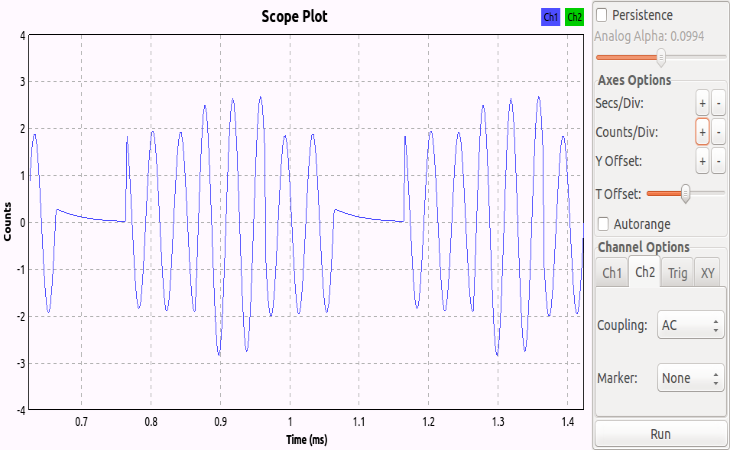
\includegraphics[width=\textwidth]{lab5/pdf/lab5_3.pdf}
\end{figure}
\end{frame}
%------------------------

\begin{frame}{Modulación BPSK en GRC}
\begin{figure}[H]
\centering
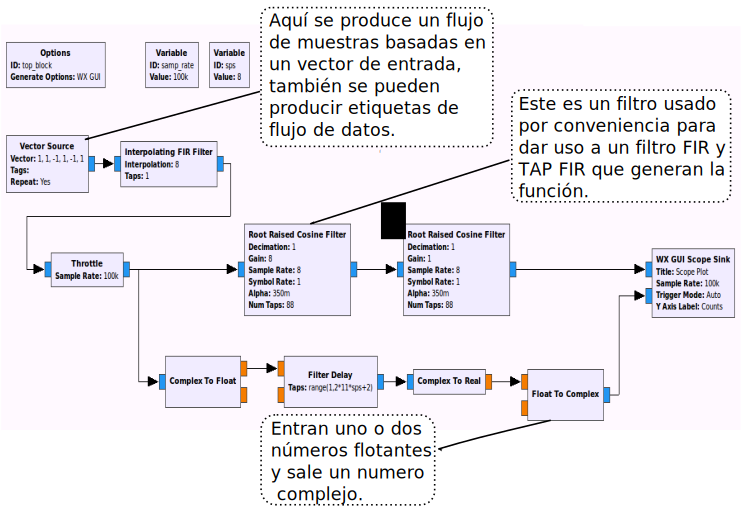
\includegraphics[width=.8\textwidth]{lab5/pdf/lab5_4.pdf}
\end{figure}
\end{frame}
%------------------------

\begin{frame}{Modulación BPSK en GRC}
\begin{figure}[H]
\centering
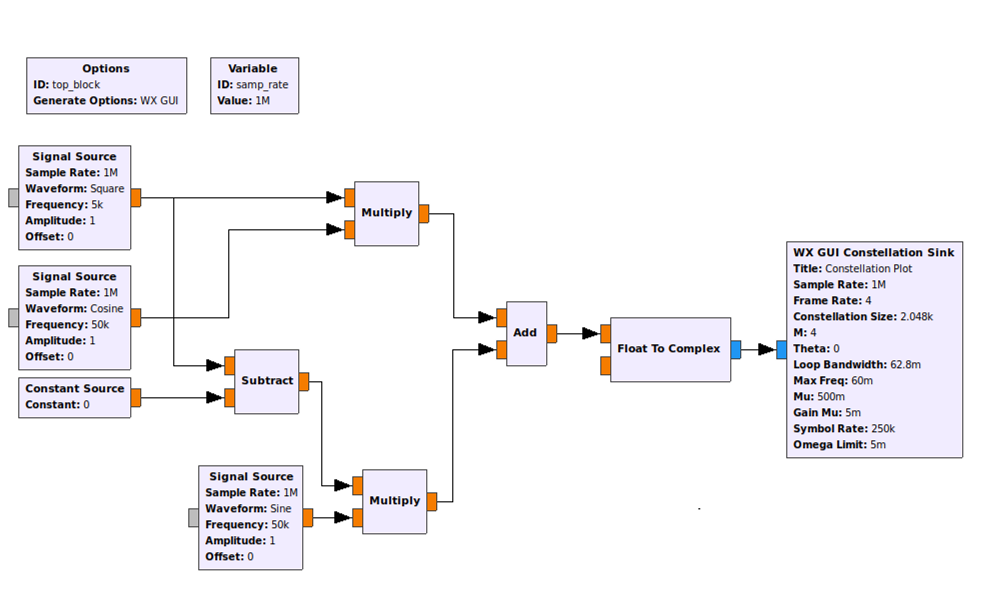
\includegraphics[width=\textwidth]{lab5/pdf/lab5_5.pdf}
\end{figure}
\end{frame}
%------------------------